\documentclass[11pt]{article}
\usepackage{amsmath,amssymb,booktabs,graphicx,hyperref,array,longtable}
\graphicspath{{research_A_horizon/figures/}{../figures/}}
\title{Preemption and Recovery Dynamics under KV Pressure\\\large An empirical study (working draft)}
\author{Author information pending}
\date{October 2026}
\begin{document}
\maketitle
\begin{abstract}
This study investigates long interruptions after the first output token in
single-GPU streaming generation under KV pressure. Historical measurements
motivate a scheduler combining admission headroom, recovery leases, and
lease-aware victim selection. The completed initial natural-EOS frontier does not improve on the best
static cap in both tail-gap and first-token latency. We therefore organize
the study around measured tradeoffs and limits of recovery interventions.
The full cross-workload and cross-model evaluation remains in progress;
no general thrash-free guarantee is established.
\end{abstract}
\section{Introduction}
Streaming inference exposes interruptions that aggregate throughput can
hide. Under KV pressure, a request may repeatedly lose its GPU state and
wait to recover after it has already produced output. Limiting concurrency
can avoid such interruptions, but moves waiting time before the first token.
The resulting design question is how admission and recovery decisions
trade first-token delay against interruptions during generation.

We study this question in a pinned single-GPU vLLM offload runtime, using
HORIZON as an executable intervention that combines bounded reservation,
recovery protection, and observed-stall ordering. The initial frontier
does not establish an advantage over a tuned static cap. Fixed-setting
transfer experiments instead show that the direction of the tradeoff
depends on the temporal concentration of prompt demand.

The evidence currently supports a scoped empirical account: recovery
waiting can dominate observed LOAD time; eliminating preemption can
increase first-token delay; and the best observed reservation setting on
one constructed workload need not dominate a fixed cap on another.
Single-run component ablations further expose a tradeoff between stall
frequency and extreme gaps. The second model, lower-budget frontier,
and independent confirmation remain necessary to establish breadth.
\section{Background}
The pinned vLLM 0.26 scheduler executes running requests before waiting
admissions. Its FCFS allocation-failure path selects the running tail.
Asynchronous offload recovery spans allocation, LOAD, completion notification,
acknowledgment, residual computation, and the next client-visible output.
\section{Characterization}
Historical B traces contain a recovery interval in which 62 peers develop
one-page deficits absent from the initial 12-page growth set. This motivates
multi-step accounting; it is not an independent validation of HORIZON.
Historical fixed-output experiments are separated from new Instruct
natural-EOS measurements. Figure~\ref{fig:motivation} uses existing B data;
Table~\ref{tab:historical} summarizes six historical narrow interventions
without treating their failures as a general impossibility result.
\IfFileExists{research_A_horizon/figures/T2/table.tex}
{\begin{table}[ht]
\centering\small
\caption{Historical narrow interventions and their limits (T2). These are fixed-output B studies, not HORIZON performance results. Source sections and metric hashes are retained in the reproduction data.}
\label{tab:historical}
\begin{tabular}{>{\raggedright\arraybackslash}p{.17\textwidth}>{\raggedright\arraybackslash}p{.34\textwidth}>{\raggedright\arraybackslash}p{.36\textwidth}}
\toprule
Intervention & Observation & Explanation and limit \\
\midrule
Full-tail reservation & ACK-to-allocation failures disappeared; whole-service effects changed sign across the two pairs. & Holding the target history did not prevent its preemption during residual computation; peer growth remained outside the reservation. \\[4pt]
Once versus repeat8 & All 16 bypasses produced output then re-preempted; selected short requests improved while bypassed long requests waited longer. & Short recovery pulses divided gaps but did not sustain service; fewer request-seconds of recovery did not imply faster completion. \\[4pt]
Bounded retry deferral & One 74 ms wait ended at a real completion; the second candidate run had no qualifying action. & The action population was narrow and mean differences preceded intervention; stable whole-service benefit was not established. \\[4pt]
Yield across ACK & Two breaks crossed ACK, but the target emitted only one token before another preemption. & A different running request exhausted capacity through decode growth; earlier ACK access did not provide continuing headroom. \\[4pt]
Unique8 versus repeat8 & Removing repeated bypasses reduced LOAD traffic but increased maxgap P99 by 35.6 and 33.1 percent. & Repeated outputs had split long gaps; suppressing those useful service pulses traded away smoothness without stable completion gains. \\[4pt]
One-donor exchange & One controlled exchange produced one target token, then re-preemption; donor flow increased by 4.31 s. & Initial T/R/G covered entry but missed later peer growth. Costs shifted to the donor and peers; one active run is not replicated evidence. \\[4pt]
\bottomrule
\end{tabular}
\end{table}
}
{\begin{table}[ht]
\centering\small
\caption{Historical narrow interventions and their limits (T2). These are fixed-output B studies, not HORIZON performance results. Source sections and metric hashes are retained in the reproduction data.}
\label{tab:historical}
\begin{tabular}{>{\raggedright\arraybackslash}p{.17\textwidth}>{\raggedright\arraybackslash}p{.34\textwidth}>{\raggedright\arraybackslash}p{.36\textwidth}}
\toprule
Intervention & Observation & Explanation and limit \\
\midrule
Full-tail reservation & ACK-to-allocation failures disappeared; whole-service effects changed sign across the two pairs. & Holding the target history did not prevent its preemption during residual computation; peer growth remained outside the reservation. \\[4pt]
Once versus repeat8 & All 16 bypasses produced output then re-preempted; selected short requests improved while bypassed long requests waited longer. & Short recovery pulses divided gaps but did not sustain service; fewer request-seconds of recovery did not imply faster completion. \\[4pt]
Bounded retry deferral & One 74 ms wait ended at a real completion; the second candidate run had no qualifying action. & The action population was narrow and mean differences preceded intervention; stable whole-service benefit was not established. \\[4pt]
Yield across ACK & Two breaks crossed ACK, but the target emitted only one token before another preemption. & A different running request exhausted capacity through decode growth; earlier ACK access did not provide continuing headroom. \\[4pt]
Unique8 versus repeat8 & Removing repeated bypasses reduced LOAD traffic but increased maxgap P99 by 35.6 and 33.1 percent. & Repeated outputs had split long gaps; suppressing those useful service pulses traded away smoothness without stable completion gains. \\[4pt]
One-donor exchange & One controlled exchange produced one target token, then re-preemption; donor flow increased by 4.31 s. & Initial T/R/G covered entry but missed later peer growth. Costs shifted to the donor and peers; one active run is not replicated evidence. \\[4pt]
\bottomrule
\end{tabular}
\end{table}
}
\begin{figure}[ht]
\centering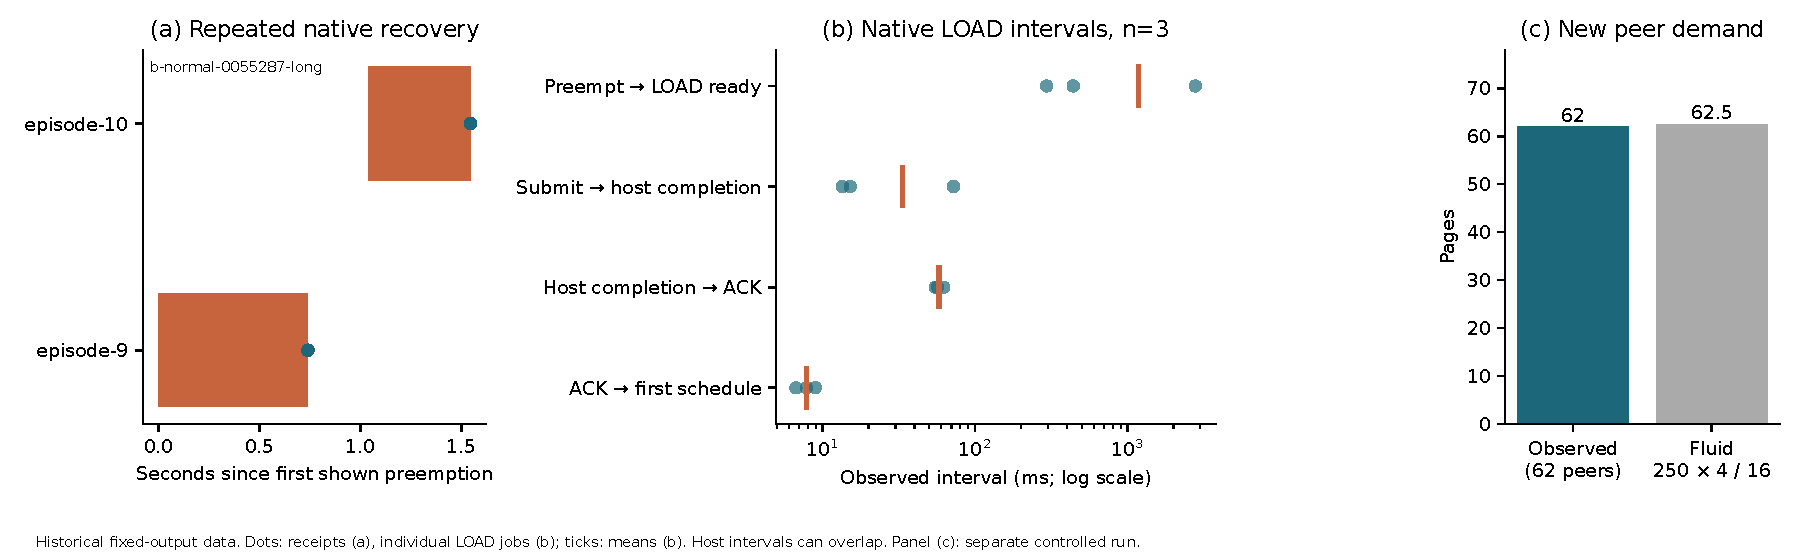
\includegraphics[width=\textwidth]{F1/F1.pdf}
\caption{Historical motivation, not a HORIZON result. (a) Two native recovery
episodes of the same request. (b) Three observed native LOAD jobs; dots show
individual host intervals and ticks their means. Intervals are not additive
GPU costs. (c) In a separate controlled recovery run, 62 peers each require
one new page after four steps; the fluid reference of 62.5 pages is explanatory
sizing, not an exact page-wise safety bound.}
\label{fig:motivation}
\end{figure}
\section{Model and Conditional Capacity Guarantee}
Let $b=16$, $N_i$ be the current known sequence extent, and $B_i$ its physically
held GPU blocks at a common allocation boundary. The fluid estimate
$D(H)=\lceil nH/b\rceil$ is useful for sizing but is not generally a page-wise
upper bound. For $n=250,H=1$ and page-aligned extents, growth is 250 blocks,
whereas $D=16$. For a fixed cohort with $B_i=\lceil N_i/b\rceil$ and $H$ a
multiple of $b$, the exact growth equals $nH/b$.

For a qualified full-attention layout without shared pages, a conservative
endpoint demand is
\[
 E(H)=\sum_{i\in S}\max\{0,\lceil\min(M,N_i+H)/b\rceil-B_i\},
\]
where $S$ includes the prospective recovered request and all owners that may
decode in the window; $M$ is the model length limit. Owners unable to decode
still require their unallocated known-history pages. Native in-flight
reservations overlapping these demands are counted once. LOAD hits reduce
recomputation, not the destination GPU footprint.

\paragraph{Conditional lemma.}
If the initial free pages cover all endpoint deficits of a fixed owner set,
each owner advances by at most one additional position per step, and no
unaccounted allocations or sharing changes occur, then decode growth cannot
exhaust that reservation within $H$ steps.
\paragraph{Proof.}
At every intermediate step each owner's required page extent is no greater
than its endpoint extent. The sum of monotone page increments is bounded by
the reserved endpoint deficits. Completions only reduce demand. \hfill$\square$

\paragraph{Dynamic capacity condition.}
Let $L_t$ be the largest remaining lifetime of any active lease and let
$E_t(L_t)$ include every running or in-flight owner. Suppose each entrant
passes an exact endpoint gate with horizon at least $L_t$, and a new lease
of length $H_r$ passes a gate covering all owners plus its target at a
horizon of at least $\max(L_t,H_r)$. Assume private pages, no unaccounted
allocations, and the same one-position-per-step extent bound as above.
Allocations must stay within their charged endpoint extents. Then
\[
F_t\ \ge\ E_t(L_t)
\]
is an invariant from the first successful lease gate until the last lease
expires, and decode growth alone cannot exhaust the covered capacity.

\paragraph{Proof.}
For an existing owner, advancing one step increases its known extent by
at most one while the remaining lease horizon decreases by one; its
charged endpoint therefore cannot increase. Allocating $x$ pages within
that endpoint decreases both free capacity and its remaining deficit by
$x$. Completion removes the owner's deficit and returns its pages.
An entrant gate re-establishes the inequality for the enlarged owner set
before charging its allocation. A new-lease gate likewise covers any
extension of the maximum remaining horizon. Induction over these events
preserves the inequality. \hfill$\square$

With fixed $H_r$ and $H_a\ge H_r$, the horizons satisfy this condition,
but only if every relevant entry is qualified and gated and all in-flight
growth remains charged. The fluid estimate alone is insufficient.
For an adaptive $H_r$, a newly shortened estimate does not shorten older
leases: the gate must still cover their largest remaining lifetime.
The prototype's UNKNOWN bypasses and adaptive-horizon path have not been
shown to satisfy this contract. Its all-leased victim fallback also
permits preemption if capacity coverage is lost. Thus this conditional
capacity result is not a global thrash-free guarantee for the implementation.
\section{Design}
HORIZON gates new admissions and recoveries using a bounded growth horizon,
orders eligible recovery prefixes by observed output stall, and prefers
victims without active leases. The native FCFS break, token quantum,
transfer concurrency, and acknowledgment protocol are retained.
\section{Implementation}
The prototype is a per-scheduler install/uninstall adapter over the pinned
native schedule method. Three CPU checks cover the 250-request, 32-step
growth scenario, execution of the transformed victim/refund branch, and
agreement with a recorded native KNOWN allocation snapshot (700 required
pages at a 32-step horizon). These are implementation checks, not serving
performance evidence. A residue histogram
permits constant-size growth queries at fixed block size. Reverse victim
search and arbitrary removal from the native Python list are linear in the
worst case; they must not be reported as constant-time operations.
The measured ledger prototype rebuilds lazily during the waiting phase.
Each rebuild visits the running/in-flight owner union and checks every held
physical block, taking $O(N+B)$ for $N$ owners and $B$ held blocks.
Recovery reentry invalidates the cache, so one waiting phase can trigger
multiple rebuilds. Only gate queries over cached totals take constant time.
This does not yet meet the intended constant-cost maintenance requirement.
Expiry-bucket and unchanged-footprint reentry optimizations have CPU
checks and are included in the queued revision \texttt{code-r13}, but not
in the measured revisions; no measured overhead benefit is attributed to
them. The common STORE
cursor intervention is wired into every arm and its cost is included.
The adapter has executed complete OLMoE-Instruct runs in the native engine.

\paragraph{Version boundary.}
The reported initial frontier and transfer runs used the original ledger.
A subsequent consistency check found that adding an asynchronous LOAD
charged its future growth, whereas rebuilding the ledger retained only its
known-history deficit until it became running. For a 16-token owner holding
one page, a 32-step growth charge therefore changed from two pages to zero
across that boundary. The corrected implementation retains endpoint demand
for the union of running and in-flight owners, counting overlapping membership
once. Its CPU checks pass, and the subsequent eight-cell ablation group
executes this correction in the native GPU engine.
This is a defect in the experimental adapter, not the pinned vLLM scheduler.
Existing results retain their original code version; the initial frontier
does not evaluate this correction, which is present in \texttt{code-r12}.

A later CPU case exposed a separate owner-accounting error: a new request
with no preemption history can already be represented as an in-flight LOAD
owner. Its subsequent entry into RUNNING could add its demand again when
a cached ledger existed. In the constructed complete-LOAD case, the
32-step charge rose incorrectly from two pages to four. Revision
\texttt{code-r13} tracks represented owners and either reuses the validated
unchanged-footprint contribution or invalidates the ledger for rebuilding.
Complete and partial LOAD CPU cases pass; GPU validation is pending.
In each of the eight \texttt{code-r12} ablation runs, 255 accepted LOAD jobs
had no earlier recorded preemption for the corresponding request. Thus new-request
LOAD is present in the measured workload, although these traces do not record
whether a cached ledger existed at each entry and do not establish the
frequency or service impact of duplicate charging. The ablation values below
remain measurements of \texttt{code-r12}, with this implementation caveat;
they are not results for \texttt{code-r13}. No historical metric is rewritten.
\section{Evaluation}
Primary metrics are request maxgap P99 and the fraction with maxgap above
200 ms. Costs include TTFT P95, output throughput, and arrival-to-completion
time. Joint goodput counts completed requests satisfying TTFT at most 5 s
and maxgap at most 200 ms over the full observation window. All arrivals,
failures, timeouts, and unfinished requests remain in the population.

\paragraph{Runtime.}
Experiments use one NVIDIA RTX PRO 6000 Blackwell Server Edition
(97,887 MiB), vLLM 0.26.0, and PyTorch 2.11.0+cu130. We use BF16,
a 4096-token maximum sequence length, a 1024-token scheduling budget,
chunked prefill, and the synchronous FCFS scheduler with asynchronous
native KV offload. GPU KV allocation is fixed explicitly to 24 or
48 GiB; host offload capacity is 16 GiB. Prefix caching is disabled.
These are equal-KV-budget comparisons, not equal total GPU footprint
across the two models.

Each cell starts a fresh engine. The standard application warmup submits
32 requests and then two requests, each with a 16-token output cap,
drains transfers, and resets connector state before measurement.
The additional diagnostic warmup is identified separately below.
Warmup does not eliminate all measurement-time compilation, whose cost
remains included. The measurement driver assigns open-loop arrival times
$i/\lambda$ from a host monotonic-clock origin. Due requests enter the
engine when the driver next runs; latency is measured from the assigned
arrival, so submission lag is included. Output gaps use host receipt
times, rather than device completion timestamps. Measurement ends when
the request cohort finishes or the 240-second deadline is reached;
post-measurement transfer draining is recorded separately. Per-cell files
retain initialization and warmup records, while group receipts retain
whole-cell duration in addition to the request measurement window.

Planned matrix: OLMoE-Instruct and Qwen3-8B, three workload families,
24/48 GiB GPU KV budgets, and native, three static caps, full-budget, MC,
and HORIZON arms. The first W2 input reuses 256 natural source documents,
alternating chat-formatted prompts of 512 and 3072 tokens, with a requested
output cap of 1024 and natural EOS enabled. The instruction asks for a
structured document analysis. This constructed development mixture is not
a production workload trace. W2 includes calibrated arrival rates $\lambda$ and
$2\lambda$. F2 is the TTFT--maxgap frontier; F3 tests fixed settings across
loads; F4 ablates leases/admission/stall order; F5 reports reservation and
scheduler cost; F6 reproduces the frontier on Qwen.

\paragraph{Model-specific inputs.}
OLMoE-Instruct uses greedy decoding. Prepared Qwen3-8B inputs use its
non-thinking chat template, temperature 0.7, top-$p$ 0.8, and top-$k$ 20.
Qwen's per-document sampling seed combines the fixed seed 20261016
with a hash of document identity, preserving that seed when W3 reorders
W2's documents. This controls the seed assignment; it does not establish
identical generated work across policies.
Tokenization yields Qwen W1 lengths of 459--512 tokens (mean 505.84),
and W2/W3 lengths of 459--3072 (mean 1781.05), with 128 requests above
512 tokens. Only 39 Qwen prompts reach exactly 3072 tokens, whereas
OLMoE W2/W3 contain 128 prompts at each of 512 and 3072 tokens.
Thus, length bounds and document identities transfer across models,
not identical token counts or calibrated pressure. Arrival rates are
calibrated separately per model and KV budget. These Qwen input facts
describe prepared assets, not completed serving measurements.

\paragraph{Initial calibration, not a policy comparison.}
At 48 GiB and 10 requests/s, the first valid native run completed all 256
requests, with 215 natural stops and 41 length-limited completions.
Eight requests were preempted (3.125\%), below the target 5--15\% pressure
range. Maxgap P99 was 1.071 s, stall rate 15.625\%, TTFT P95 16.537 s,
mean completion time 35.170 s, and output throughput 2613.45 tokens/s.
The next rate was 20 requests/s. An initialization failure caused by a missing
historical sampler environment setting is retained separately; it contributes
no measured requests. A measurement-time kernel JIT warning in the valid run
is retained, with no post-hoc time subtraction. No HORIZON benefit is yet
established.
At 24 GiB, the native run at 10 requests/s preempted 39/256 requests
(15.23\%), just above the calibration band. Halving the arrival rate to
5 requests/s yielded 26/256 (10.16\%), selecting $\lambda=5$ and
$2\lambda=10$ for this budget. All 256 requests completed: 216 natural
stops and 40 length-limited completions. Maxgap P99 was 1.055 s,
stall rate 19.14\%, TTFT P95 13.016 s, mean flow 26.472 s, and
throughput 2211.93 tokens/s. This calibration includes measurement-time
JIT cost and is not a policy comparison. Its 28 asynchronous recovery
episodes all contain the newly recorded ACK-application and reentry
allocation boundaries; this validates observation coverage for this run,
not HORIZON's recovery gate.
\paragraph{First paired development result.}
At 20 requests/s, native preempted 17 of 256 requests (6.64\%), selecting
$\lambda=20$ for this model, workload, and budget. Both native and
HORIZON $(H_a,H_r)=(64,32)$ completed all requests. Maxgap P99 was
11.995 versus 7.513 s, while stall rate increased from 12.89\% to 14.84\%.
TTFT P95 was 26.822 versus 26.446 s, throughput 2698.64 versus
2668.23 tokens/s, and mean flow 39.570 versus 40.554 s. Observed
re-preemptions within 16 outputs after recovery allocation decreased from
four to zero. No lease-aware victim skips were recorded, so these data
do not establish that component's benefit. Natural-stop/length-limited
counts were 221/35 versus 219/37; generation work was not identical.
This single development pair shows a tradeoff, not dominance or a
confirmed policy improvement. Native repetitions and tuned-cap comparisons
are reported below. Whole-scheduler host time was 1175 versus 1493
$\mu$s/step, including the configured instrumentation.

Full-budget and MC baselines reuse the existing C policy sources and
installers. The current MC adapter uses the synchronous scheduled-prefill
qualification path; it is not a reproduction of C's asynchronous v25
engine. Both initial baseline runs completed all 256 requests with zero
preemptions and zero native-fit prediction mismatches over 511 checks each.
Full-budget yielded maxgap P99 0.547 s and TTFT P95 30.719 s. The MC
adapter rejected all 640 candidate relaxations because the new target used
external KV loading; its future-peak rule never acted. This result cannot
establish the performance of an active MC policy.

Thirty full-budget requests shared the same 0.547 s output-gap interval
early in measurement, alongside a fused-MoE JIT warning. This supports a
common startup disturbance, not 30 independent recovery events. Existing
measurements retain this cost. A separate broader-shape warmup group still
exhibited measurement-time JIT and did not eliminate the shared disturbance.
Its native run overlapped model downloading, and overlap could not be
excluded for its full-budget run; both are diagnostic rather than clean
confirmation. These runs are not pooled with the legacy-warmup frontier.
The same group also exercised an MC component adapted to external LOAD
targets, recording 117 successful relaxations in 603 evaluations. That arm
ran after downloading was suspended and completed without preemption, but
the group's limitations prevent attributing a clean comparative benefit.
\paragraph{Observed recovery boundaries.}
Joining the first development pair by request and LOAD job yields 22 native
and 11 HORIZON recovery episodes. Native median preemption-to-allocation
wait was 3.905 s, versus 0.277 s from allocation to the next output;
the LOAD submission-to-host-notification median was 0.072 s. Corresponding
HORIZON medians were 6.666, 0.335, and 0.045 s. These are different,
policy-selected episode populations, not independent system repetitions
or a matched causal comparison. The intervals suggest that transfer time
alone is an incomplete account of these stalls. ACK-application timestamps
were not recorded in these traces and remain missing; host notification
is not device completion, and medians of overlapping intervals are not
summed into a synthetic recovery duration.
\begin{figure}[ht]
\centering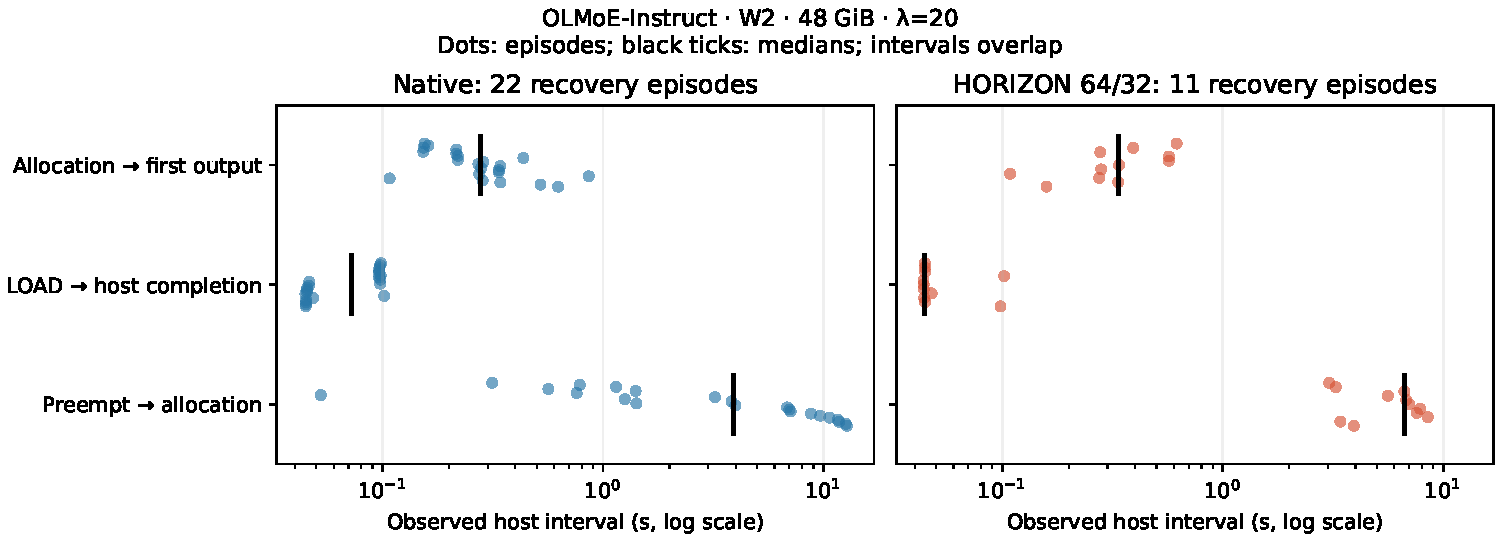
\includegraphics[width=\textwidth]{F1/recovery.pdf}
\caption{Observed recovery intervals for the initial Instruct runs.
Dots represent 22 native and 11 HORIZON recovery episodes; black ticks
show medians. These policy-selected populations are not matched causal
comparisons or independent experimental repetitions. The allocation-to-output
interval overlaps LOAD service; intervals must not be added. ACK and
reentry timestamps were unavailable and are omitted.}
\label{fig:instruct-recovery}
\end{figure}

The later native 24 GiB calibration records all seven host boundaries
for its 28 recovery episodes, each with one accepted LOAD
(Figure~\ref{fig:complete-recovery}). Their mean preemption-to-output
duration is 0.589 s: 0.474 s precedes the first allocation, while
LOAD submission to host completion contributes 0.054 s. This separates
queueing before allocation from transfer notification and subsequent
resumption. The six adjacent intervals sum to the observed total for
every episode; this is a descriptive decomposition of one run, not
an independent-repeat estimate or a causal policy comparison.
\begin{figure}[ht]
\centering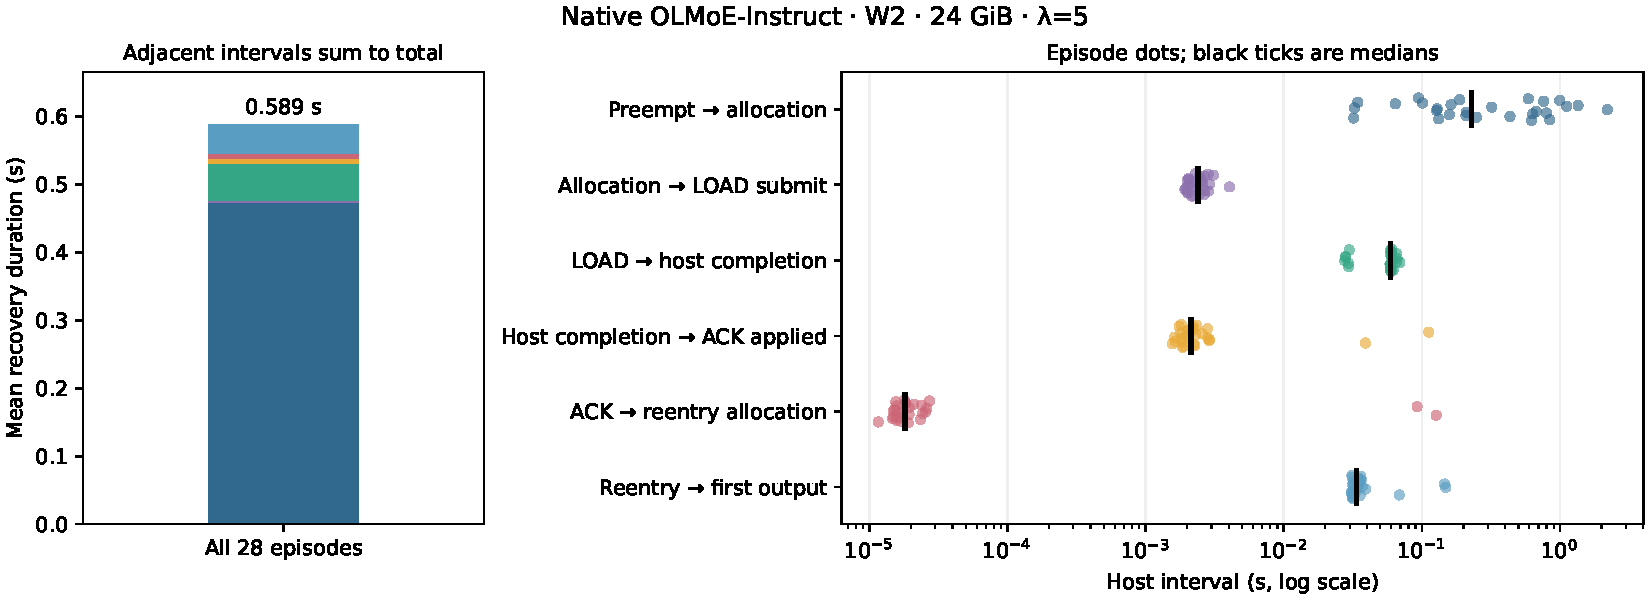
\includegraphics[width=\textwidth]{F1/complete-chain.pdf}
\caption{Complete host recovery chains in the native 24 GiB, $\lambda=5$
calibration. Left: mean duration partitioned into six adjacent intervals,
with colors corresponding to the right-hand rows. Right: all 28 episodes
and their interval medians. ACK application and reentry allocation are
observed explicitly; host notification does not measure device completion.
Unlike Figure~\ref{fig:instruct-recovery}, these intervals do not overlap.}
\label{fig:complete-recovery}
\end{figure}

\paragraph{Local native repetitions.}
Three subsequent native runs at the selected working point all completed
256 requests. Their maxgap P99 values were 16.261, 15.048, and 12.204 s;
stall rates were 17.19\%, 14.45\%, and 21.09\%. Mean flow was 41.134,
40.298, and 40.133 s, with throughput 2653.55, 2672.49, and 2672.87
tokens/s. The first HORIZON run's mean flow and throughput fall within
these observed native values and are treated as indistinguishable at
this stage. The earlier paired stall increase is not a stable inferred
policy effect. These three runs describe local variability, not a
transferable noise floor or a significance threshold.
\begin{figure}[ht]
\centering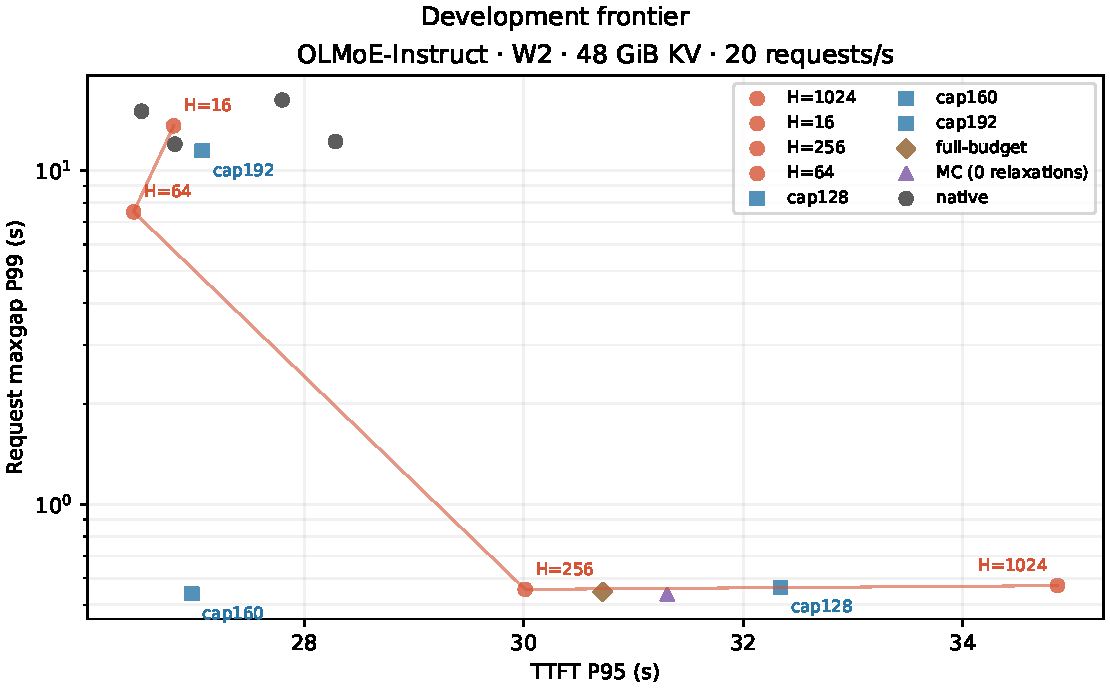
\includegraphics[width=.9\textwidth]{F2/F2.pdf}
\caption{Complete initial development frontier under legacy warmup. Each mark is one
complete run; native includes calibration and three subsequent repetitions.
HORIZON marks are available horizon settings at $H_r=32$. MC recorded
zero admission relaxations and therefore exercised its full-budget fallback. All planned initial arms are shown. No confidence interval or
confirmed dominance is claimed.}
\label{fig:frontier}
\end{figure}

The additional workload families retain the document-analysis instruction.
W1 truncates all source prefixes to at most 512 chat tokens. W3 retains
W2's documents and prompt-length mixture but groups the long requests
before the short requests, changing temporal demand concentration.
No short document is padded or repeated to fabricate a long request.
These inputs remain diagnostic constructions, not deployment traces.
The generated W3 prompt multiset exactly matches W2 by document identity.

\paragraph{Fixed-setting transfer.}
With cap160 and $H_a=256,H_r=32$ fixed after W2 tuning,
W1 stall rates were both 12.891\%, while TTFT P95 was 11.181 versus
0.186 s. At twice the W2 arrival rate, cap160 retained zero preemptions,
whereas HORIZON preempted four requests; maxgap P99 was 0.557 versus
3.967 s. Under W3's concentrated long arrivals, cap160 preempted 22
requests and HORIZON none. Stall rates were 7.8125\% versus 0.3906\%,
and TTFT P95 36.948 versus 32.129 s. However, W3 mean completion time
was 46.282 versus 47.578 s. These single-run results indicate workload-dependent
tradeoffs, not load-independent superiority. Natural-stop/length-limit
counts differ (W3: 224/32 versus 214/42); equal generation work and
quality are not established. Startup JIT costs remain included.
\begin{figure}[ht]
\centering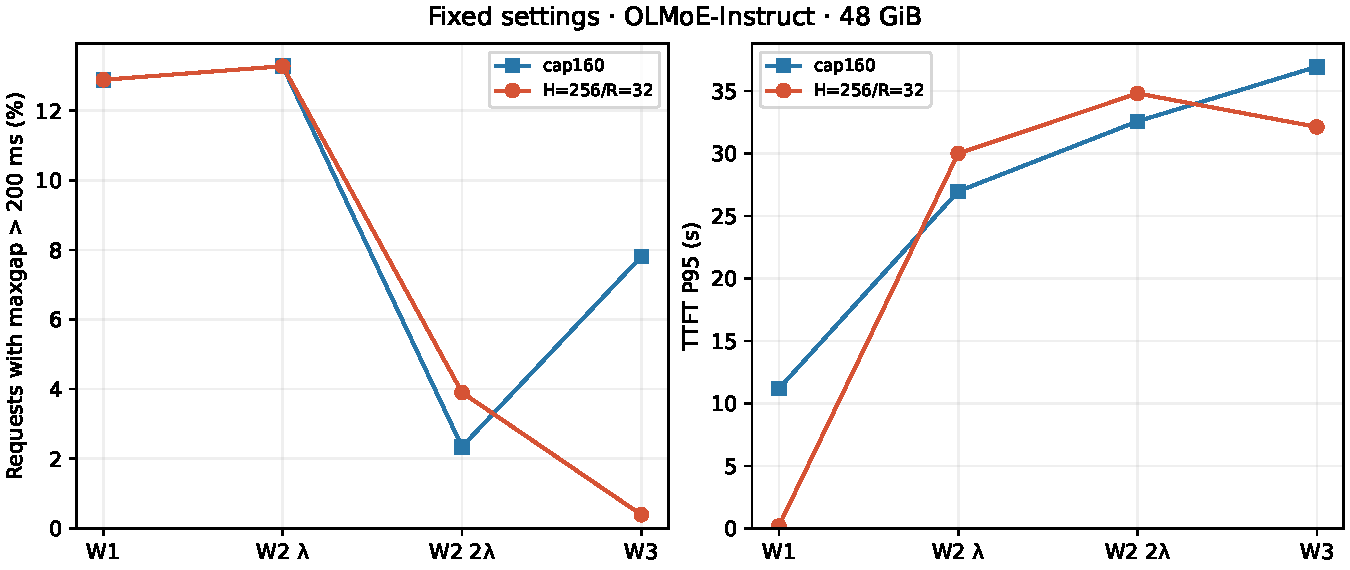
\includegraphics[width=\textwidth]{F3/F3.pdf}
\caption{Fixed cap160 and HORIZON256/32 across workloads at 48 GiB.
W2 $\lambda$ reuses tuning data; remaining points are single transfer runs.
Settings are unchanged. No uncertainty intervals or universal advantage
are inferred. All runs use natural EOS and legacy warmup.}
\label{fig:transfer}
\end{figure}

\paragraph{Initial frontier.}
All three static caps and four horizon settings completed. Cap160 had
zero preemptions, TTFT P95 26.975 s, and maxgap P99 0.540 s.
HORIZON at $H_a=16$ yielded 26.811 s and 13.607 s; at $H_a=256$,
30.013 s and 0.556 s; at $H_a=1024$, 34.864 s and 0.570 s.
The last two runs completed after data-disk expansion, both without
preemptions. Thus the initial HORIZON curve does not dominate the best
static cap: small horizons retain large gaps, whereas larger horizons
pay more first-token delay. Following the specified decision rule, the
paper now targets an empirical study of preemption--recovery dynamics.
These are development runs, with a shared measurement-time JIT disturbance;
they do not establish statistical dominance or general impossibility.
The remaining matrix, independent confirmation, and second model will test
how far this observed tradeoff transfers, with all outcomes retained.
\begin{figure}[ht]
\centering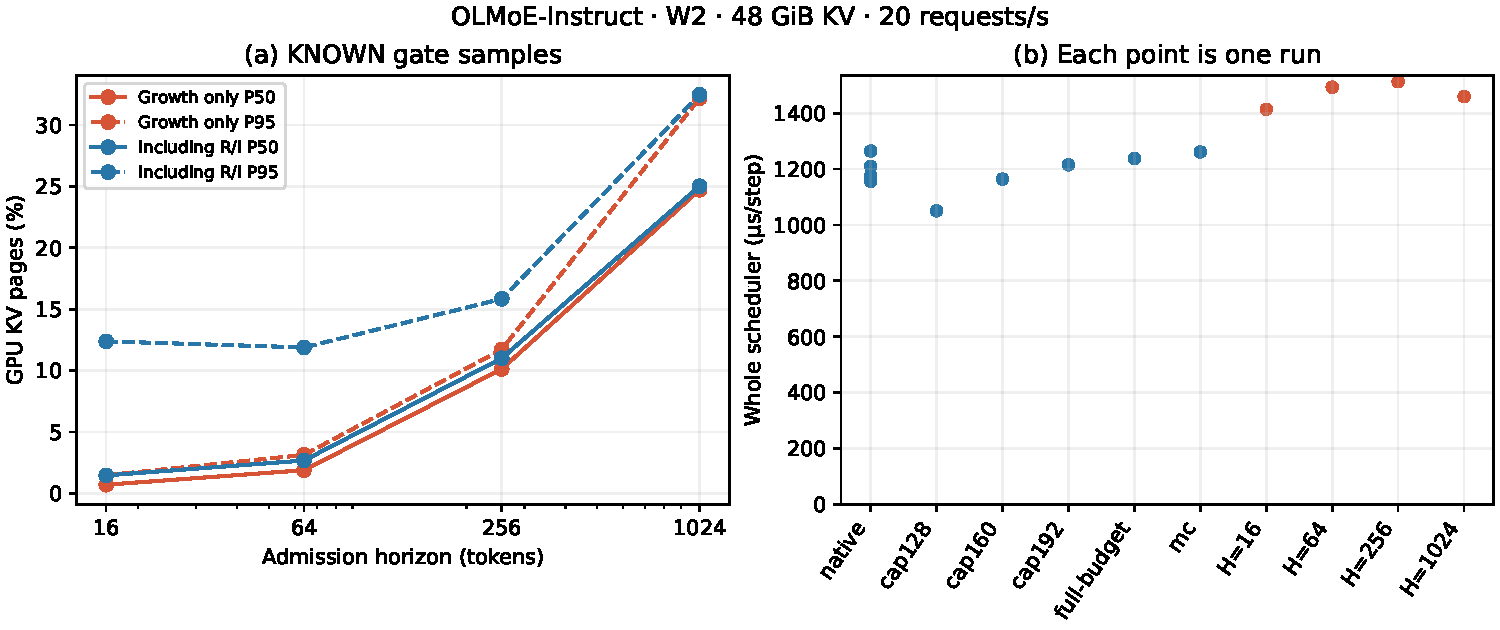
\includegraphics[width=\textwidth]{F5/F5.pdf}
\caption{Initial reservation and scheduler-cost measurements. Left: P50/P95
of KNOWN waiting-gate samples, not uniform time samples or confidence
intervals. Right: whole-scheduler mean time per step for each run, including
instrumentation. Different trajectories prevent interpreting differences
as isolated hook overhead. All points use legacy warmup.}
\label{fig:cost}
\end{figure}
HORIZON's measured scheduler means span 1414--1513 $\mu$s/step;
native cap256 runs span 1156--1265 $\mu$s/step. Growth-only reservation
medians rise from 0.696\% at $H_a=16$ to 24.723\% at $H_a=1024$.
These measurements include ledger reconstruction and per-block validation;
constant-cost maintenance has not been demonstrated.

\paragraph{Component ablations.}
All eight runs in the \texttt{code-r12} group completed 256 requests.
This revision includes the in-flight growth correction but retains the
new-request LOAD accounting risk described above.
At $H_a=64,H_r=32$, the full policy yielded maxgap P99 10.162 s,
stall rate 13.28\%, and TTFT P95 30.027 s
(Figure~\ref{fig:ablations}). Disabling recovery protection---both the
$H_r$ gate and lease-aware victim selection---reduced maxgap P99 to
5.942 s but raised stall rate to 16.80\%; TTFT P95 was 30.140 s.
Thrash counts were zero versus six. No lease-aware victim skips occurred
in the full run, so this contrast does not establish a benefit from
victim protection itself. Disabling admission produced 12.804 s maxgap
P99, 19.53\% stalls, and 26.662 s TTFT P95; disabling stall ordering
produced 12.318 s, 17.97\%, and 29.210 s, respectively.
These are one-run development contrasts, not additive component effects
or estimates of statistical significance. Output termination also differed:
the full run had 208 natural stops and 48 length-limited completions,
versus 217/39 with recovery protection disabled.
A post-hoc split by the fixed 512/3072-token prompt classes (128 requests
each) shows the same direction in both classes. The full policy's stall
rate was 13.28\% in each class, versus 16.41\% and 17.19\% without
recovery protection. However, its class-specific gap P99 values were
9.749/10.237 s versus 5.118/6.135 s. Long prompts reached the output
limit in 43 versus 36 cases. Request, prompt, document, and arrival
identities match across arms, but generated work differs; the class split
does not isolate a scheduling effect or provide independent repetitions.
\begin{figure}[ht]
\centering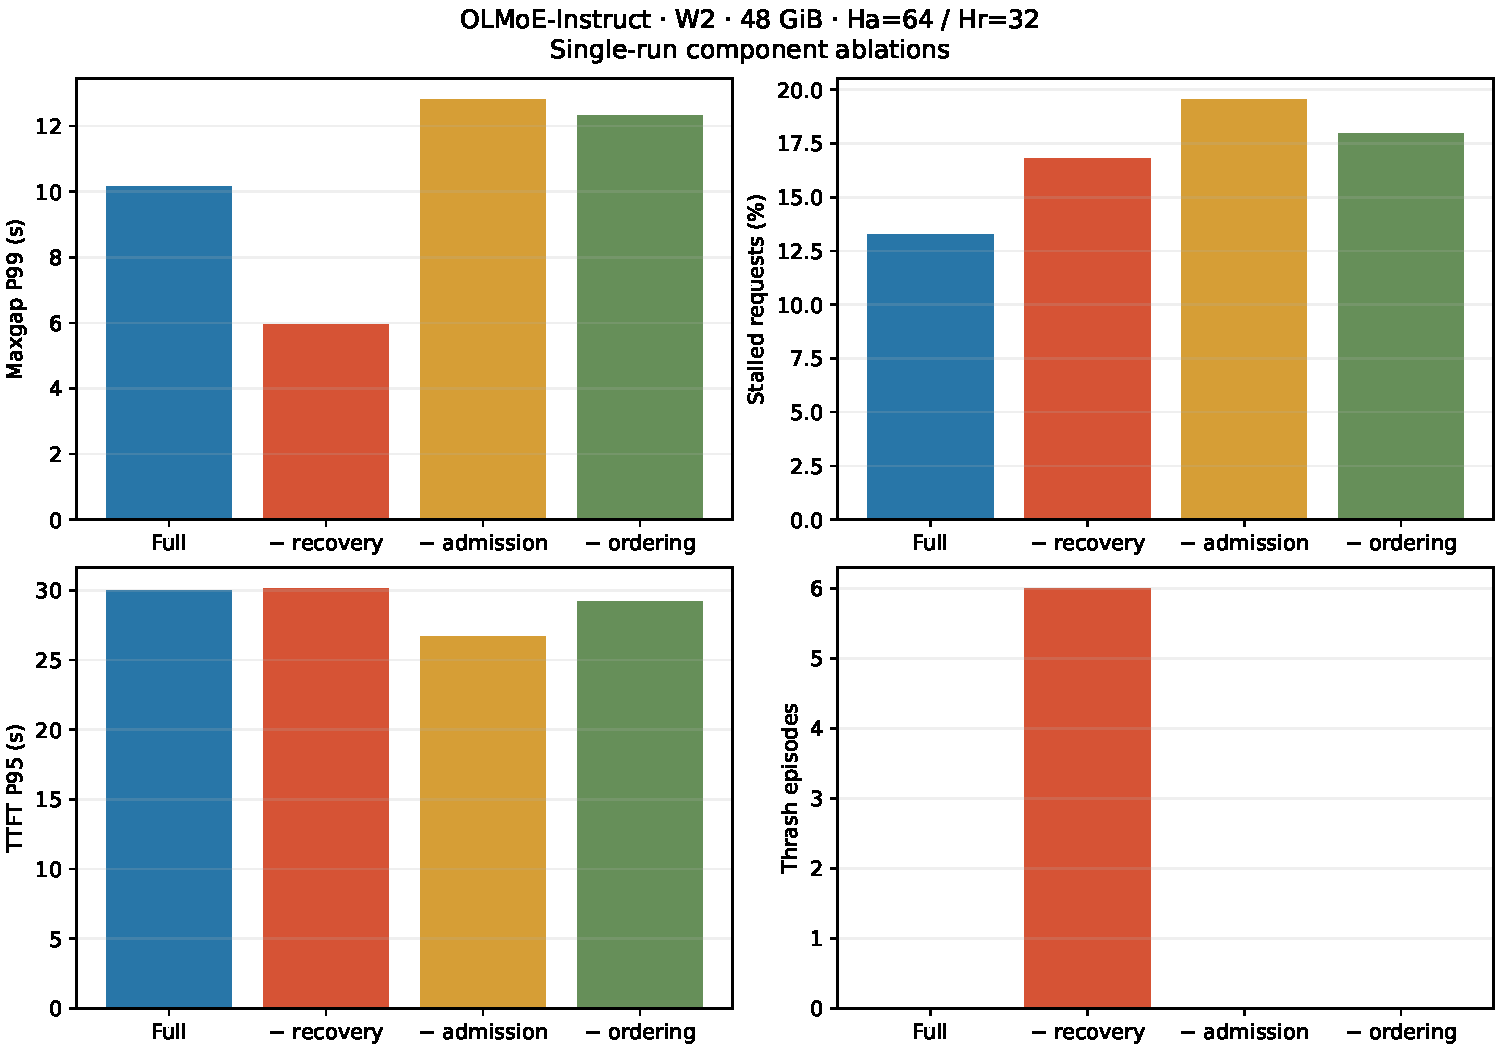
\includegraphics[width=\textwidth]{F4/F4.pdf}
\caption{\texttt{code-r12} component ablations at the event-rich
$H_a=64,H_r=32$ setting. Recovery removal disables both its gate and
victim protection. Each bar is one complete run; uncertainty across
independent runs is not estimated.}
\label{fig:ablations}
\end{figure}
The $H_r=16$, $H_r=64$, and EWMA variants yielded maxgap P99
6.237, 10.376, and 8.584 s, with stall rates 12.89\%, 11.33\%,
and 16.41\%. These observations do not identify a uniformly best
recovery horizon. The separate MC LOAD component baseline recorded
117 successful relaxations and zero preemptions, with 0.576 s maxgap
P99, 10.94\% stalls, and 26.308 s TTFT P95. Its 222/34 termination
split differs from the full policy. The results motivate comparison
against this active simple baseline across the remaining workloads;
they do not establish global dominance. Measurement-time JIT costs
remain included throughout.

\section{Related Work}
Table~\ref{tab:prior} compares the actions of nine related systems and
models. It is a source-based comparison, not a claim that all nine have
been reproduced. In particular, the measured MC arm adapts a future-peak
feasibility component while retaining FIFO; it omits MC-SF's shortest-first
subset selection. Its failure or success cannot establish the performance
of the complete original algorithm.

Protection from repeated switching and memory safety margins already
appear in prior work. UniBoost's MemGuard protects dispatched jobs until
the next service threshold, while Nested WAIT introduces a safety buffer
for unknown output lengths. Consequently, a lease or headroom signal
alone is insufficient to establish novelty. Our current contribution
hypothesis is empirical: characterize recovery losses and tradeoffs in a
pinned native offload runtime, with the applicability limits measured
across workloads and models. These broader measurements remain pending.
\IfFileExists{research_A_horizon/figures/T3/table.tex}
{\begingroup\small\setlength{\tabcolsep}{3pt}\renewcommand{\arraystretch}{1.15}
\begin{longtable}{>{\raggedright\arraybackslash}p{.14\textwidth}>{\raggedright\arraybackslash}p{.38\textwidth}>{\raggedright\arraybackslash}p{.39\textwidth}}
\caption{Prior-work actions and comparison boundaries. Names link to the primary sources; versions and locators are recorded in T3/data.json.}\label{tab:prior}\\
\toprule Method & State and action & Boundary of this comparison \\ \midrule\endfirsthead
\toprule Method & State and action & Boundary of this comparison \\ \midrule\endhead
\href{https://arxiv.org/html/2502.07115v5}{MC-SF} & Keep admitted jobs running; select waiting jobs using predicted upper lengths and future memory feasibility. & Targets total completion latency in a non-preemptive round model. Our FIFO peak adapter omits shortest-first subset selection; it is not full MC-SF. \\
\href{https://arxiv.org/abs/2504.11320v4}{WAIT} & Gate admission with fluid-guided thresholds; Nested WAIT regulates decode segments and adds a memory safety buffer. & Known-length and unknown-length variants target stability and latency. Memory headroom is prior art; our measurements concern native offload recovery. \\
\href{https://arxiv.org/abs/2404.16283}{Andes} & Prioritize and preempt at token boundaries using expected user-experience gain and GPU resource demand. & Targets smooth streaming and prompt first output. Our fixed maxgap/stall metrics do not reproduce its reading-aware utility. \\
\href{https://arxiv.org/abs/2305.05920}{FastServe} & Use skip-join multilevel feedback queues initialized from prompt length, with token-level preemption and proactive host/GPU state movement. & Targets job latency through priority and execution quanta. HORIZON retains native quanta and changes admission/recovery/victim decisions. \\
\href{https://arxiv.org/html/2411.18424v1}{FastSwitch} & Group KV blocks, adapt synchronous/asynchronous swaps, and reuse valid CPU KV copies to reduce switching cost. & Changes layout and transfer execution for fairness-aware serving. Our fixed native transfer path cannot reproduce its system-level benefit. \\
\href{https://arxiv.org/html/2606.18431v1}{UniBoost} & Unify prefill/decode priorities from arrival and attained work; quantize revisions and protect a dispatched request until its next service threshold. & MemGuard already provides minimum-run protection. Our step-based lease and peer-growth gate are a different implementation, not proof of novelty or superiority. \\
\href{https://arxiv.org/html/2601.20309v1}{SuperInfer} & Rotate requests by SLO-derived virtual lag under a transfer budget; overlap full-duplex KV movement with computation. & Designed for GH200 HBM/Grace memory and C2C transfers. Its proactive rotary scheduling and transfer engine are not reproduced by our single-GPU adapter. \\
\href{https://www.usenix.org/conference/osdi24/presentation/sun-biao}{Llumnix} & Reschedule running requests across model instances using live migration for load balancing, isolation, and priority. & Requires multiple instances and migration. Our experiment has one serving GPU; its remaining loss does not test distributed rescheduling. \\
\href{https://arxiv.org/abs/2309.06180}{vLLM} & Allocate KV in pages and share blocks to reduce fragmentation and duplicate storage. & The original paper motivates memory management. Native victim/LOAD/ACK behavior here is established from pinned 0.26 source, not attributed to the 2023 paper. \\
\bottomrule\end{longtable}
\endgroup
}
{\begingroup\small\setlength{\tabcolsep}{3pt}\renewcommand{\arraystretch}{1.15}
\begin{longtable}{>{\raggedright\arraybackslash}p{.14\textwidth}>{\raggedright\arraybackslash}p{.38\textwidth}>{\raggedright\arraybackslash}p{.39\textwidth}}
\caption{Prior-work actions and comparison boundaries. Names link to the primary sources; versions and locators are recorded in T3/data.json.}\label{tab:prior}\\
\toprule Method & State and action & Boundary of this comparison \\ \midrule\endfirsthead
\toprule Method & State and action & Boundary of this comparison \\ \midrule\endhead
\href{https://arxiv.org/html/2502.07115v5}{MC-SF} & Keep admitted jobs running; select waiting jobs using predicted upper lengths and future memory feasibility. & Targets total completion latency in a non-preemptive round model. Our FIFO peak adapter omits shortest-first subset selection; it is not full MC-SF. \\
\href{https://arxiv.org/abs/2504.11320v4}{WAIT} & Gate admission with fluid-guided thresholds; Nested WAIT regulates decode segments and adds a memory safety buffer. & Known-length and unknown-length variants target stability and latency. Memory headroom is prior art; our measurements concern native offload recovery. \\
\href{https://arxiv.org/abs/2404.16283}{Andes} & Prioritize and preempt at token boundaries using expected user-experience gain and GPU resource demand. & Targets smooth streaming and prompt first output. Our fixed maxgap/stall metrics do not reproduce its reading-aware utility. \\
\href{https://arxiv.org/abs/2305.05920}{FastServe} & Use skip-join multilevel feedback queues initialized from prompt length, with token-level preemption and proactive host/GPU state movement. & Targets job latency through priority and execution quanta. HORIZON retains native quanta and changes admission/recovery/victim decisions. \\
\href{https://arxiv.org/html/2411.18424v1}{FastSwitch} & Group KV blocks, adapt synchronous/asynchronous swaps, and reuse valid CPU KV copies to reduce switching cost. & Changes layout and transfer execution for fairness-aware serving. Our fixed native transfer path cannot reproduce its system-level benefit. \\
\href{https://arxiv.org/html/2606.18431v1}{UniBoost} & Unify prefill/decode priorities from arrival and attained work; quantize revisions and protect a dispatched request until its next service threshold. & MemGuard already provides minimum-run protection. Our step-based lease and peer-growth gate are a different implementation, not proof of novelty or superiority. \\
\href{https://arxiv.org/html/2601.20309v1}{SuperInfer} & Rotate requests by SLO-derived virtual lag under a transfer budget; overlap full-duplex KV movement with computation. & Designed for GH200 HBM/Grace memory and C2C transfers. Its proactive rotary scheduling and transfer engine are not reproduced by our single-GPU adapter. \\
\href{https://www.usenix.org/conference/osdi24/presentation/sun-biao}{Llumnix} & Reschedule running requests across model instances using live migration for load balancing, isolation, and priority. & Requires multiple instances and migration. Our experiment has one serving GPU; its remaining loss does not test distributed rescheduling. \\
\href{https://arxiv.org/abs/2309.06180}{vLLM} & Allocate KV in pages and share blocks to reduce fragmentation and duplicate storage. & The original paper motivates memory management. Native victim/LOAD/ACK behavior here is established from pinned 0.26 source, not attributed to the 2023 paper. \\
\bottomrule\end{longtable}
\endgroup
}
\section{Conclusion}
Completion requires a runnable adapter and measurements of service
tradeoffs. The initial frontier did not improve on the best static cap in both
primary frontier dimensions. The paper now develops an empirical
characterization with complete outcomes and explicit applicability limits;
the remaining experimental matrix is not yet complete.
\end{document}
